\documentclass[11pt, a4paper]{article}
\usepackage{graphicx}
\usepackage{amsmath}
\usepackage{listings}


\title{Assignment No 9} % Title

\author{Harshavardhan Mudadala \\ EE20B084} % Author name

\date{\today} % Date for the report
\begin{document}		
		
\maketitle % Insert the title, author and date

\section{Questions}
\subsection{Question 2}
In this question, we shall plot the FFT of $cos^3(0.86t)$
The FFT without the hamming Window:
\begin{figure}[h!]
\centering
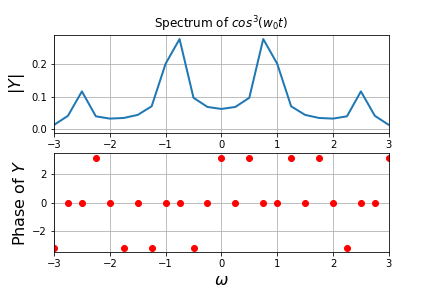
\includegraphics[scale=0.7]{fig1.png}
\label{fig:universe}
\end{figure}
\clearpage
The FFT with the hamming Window:
\begin{figure}[h!]
\centering
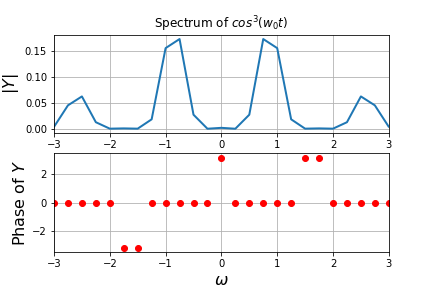
\includegraphics[scale=0.7]{fig2.png}
\label{fig:universe}
\end{figure}

We notice that a lot of the energy is stored in frequencies that aren't a part of the signal. After windowing, these frequencies are attenuated and hence the peaks are sharper in the windowed function. 

\subsection{Question 3}
We need to estimate $\omega$ and $\delta$ for a signal $\cos(\omega t + \delta)$ for 128 samples between $[-\pi,\pi)$. We estimate omega using a weighted average. We have to extract the digital spectrum of the signal and find the two peaks at $\pm\omega_0$, and estimate $\omega$ and $\delta$.
\begin{figure}[h!]
\centering
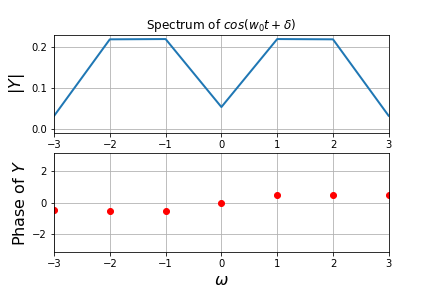
\includegraphics[scale=0.7]{fig3.png}
\caption{Fourier transform of $cos(1.5t+0.5)$}
\label{fig:universe}
\end{figure}

We estimate omega by performing a Mean average of $\omega$ over the magnitude of $|Y(j\omega)|$.
For delta we consider a widow on each half of $\omega$ (split into positive and negative values) and extract their mean slope. 

\subsection{Question 4}
We repeat the exact same process as question 3 but with noise added to the original signal.
\begin{figure}[h!]
\centering
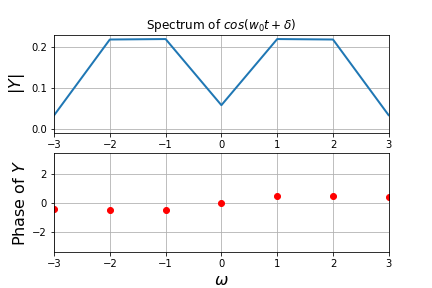
\includegraphics[scale=0.7]{fig4.png}
\caption{Fourier transform of noise + $cos(1.5t+0.5)$}
\label{fig:universe}
\end{figure}

\newpage
\subsection{Question 5}
In this question we analyze a chirp signal which is an FM signal where frequency is directly proportional to time.
A chirp signal we shall consider is given by 
\begin{equation}
    f(t) = cos(16t(1.5 + \frac{t}{2\pi}))
\end{equation}
The FFT of the chirp is given by:
We note that the frequency response is spread between 5-50 rad/s. A large section of this range apears due to Gibbs phenomenon. On windowing, only frequencies between 16 and 32 rad/s remain.
\begin{figure}[h!]
\centering
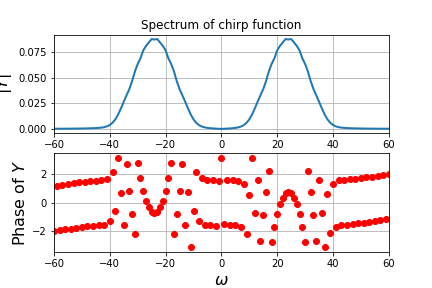
\includegraphics[scale=0.7]{fig5.png}
\caption{Chirp function fourier transform, windowed}
\label{fig:universe}
\end{figure}
\begin{figure}[h!]
\centering
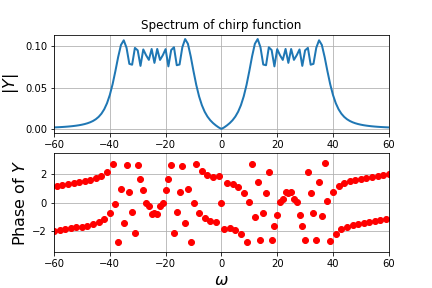
\includegraphics[scale=0.7]{fig6.png}
\caption{Chirp function fourier transform}
\label{fig:universe}
\end{figure}
\newpage
\subsection{Question 6}
For the same chirped signal, we break the 1024 vector into pieces that are 64 samples wide.
Extract the DFT of each and store as a column in a 2D array. Then plot the array as a surface plot to show how the frequency of the signal varies with time.


\begin{figure}[h!]
\centering
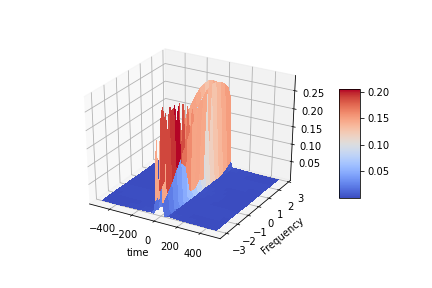
\includegraphics[scale=0.7]{fig7.png}
\caption{Chopped Chirp function, |Fourier transform|,windowed}
\label{fig:universe}
\end{figure}

\begin{figure}[h!]
\centering
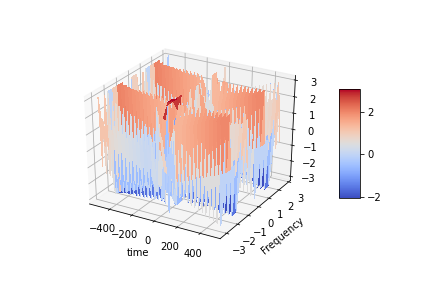
\includegraphics[scale=0.7]{fig8.png}
\caption{Chopped Chirp function, Phase of Fourier transform}
\label{fig:universe}
\end{figure}

\newpage


\end{document}